\documentclass[a4paper, 12pt]{article}
\usepackage[utf8]{inputenc}
\usepackage[english,russian]{babel}
\usepackage[warn]{mathtext}
\usepackage{graphicx}
\usepackage{float}
\restylefloat{table}
\usepackage{amsmath}
\usepackage{floatflt}
\usepackage[T2A]{fontenc}
\usepackage[left=20mm, top=20mm, right=20mm, bottom=20mm, footskip=10mm]{geometry}

\tolerance 1414
\hbadness 1414
\emergencystretch 1.5em
\hfuzz 0.3pt        % размер максимального переполнения без warning'a
\widowpenalty=10000 % запрещает одиночную строку абзаца в начале страницы
\vfuzz \hfuzz
\raggedbottom       % если на странице мало содержимого, добавить пустое место в конце, а не в середине страницы



\begin{document}

\begin{titlepage}
	\centering
	\vspace{5cm}
	{\scshape\LARGE московский физико-технический институт (национальный исследовательский университет) \par}
	\vspace{6cm}
	{\scshape\Large Лабораторная работа 3.4.5 \par}
	{\huge\bfseries Петля гистерезиса \par}
	\vspace{1cm}
	\vfill
\begin{flushright}
	{\large Б03-102}\par
	\vspace{0.3cm}
	{\LARGE Куланов Александр}
\end{flushright}
	

	\vfill


	Долгопрудный, 2022 г.
\end{titlepage}

\begin{itemize}
	\item \textbf{Цель работы:} изучение петель гистерезиса различных ферромагнитных материалов в переменных полях.
    \item \textbf{В работе используются:} автотрансформатор, понижающий трансформатор, интегрирующая цепочка, амперметр, 
    вольтметр, электронный осциллограф, делитель напряжения, тороидальные образцы с двумя обмотками.
\end{itemize}

\section{Экспериментальная установка}

\begin{figure}[h]
    \centering
    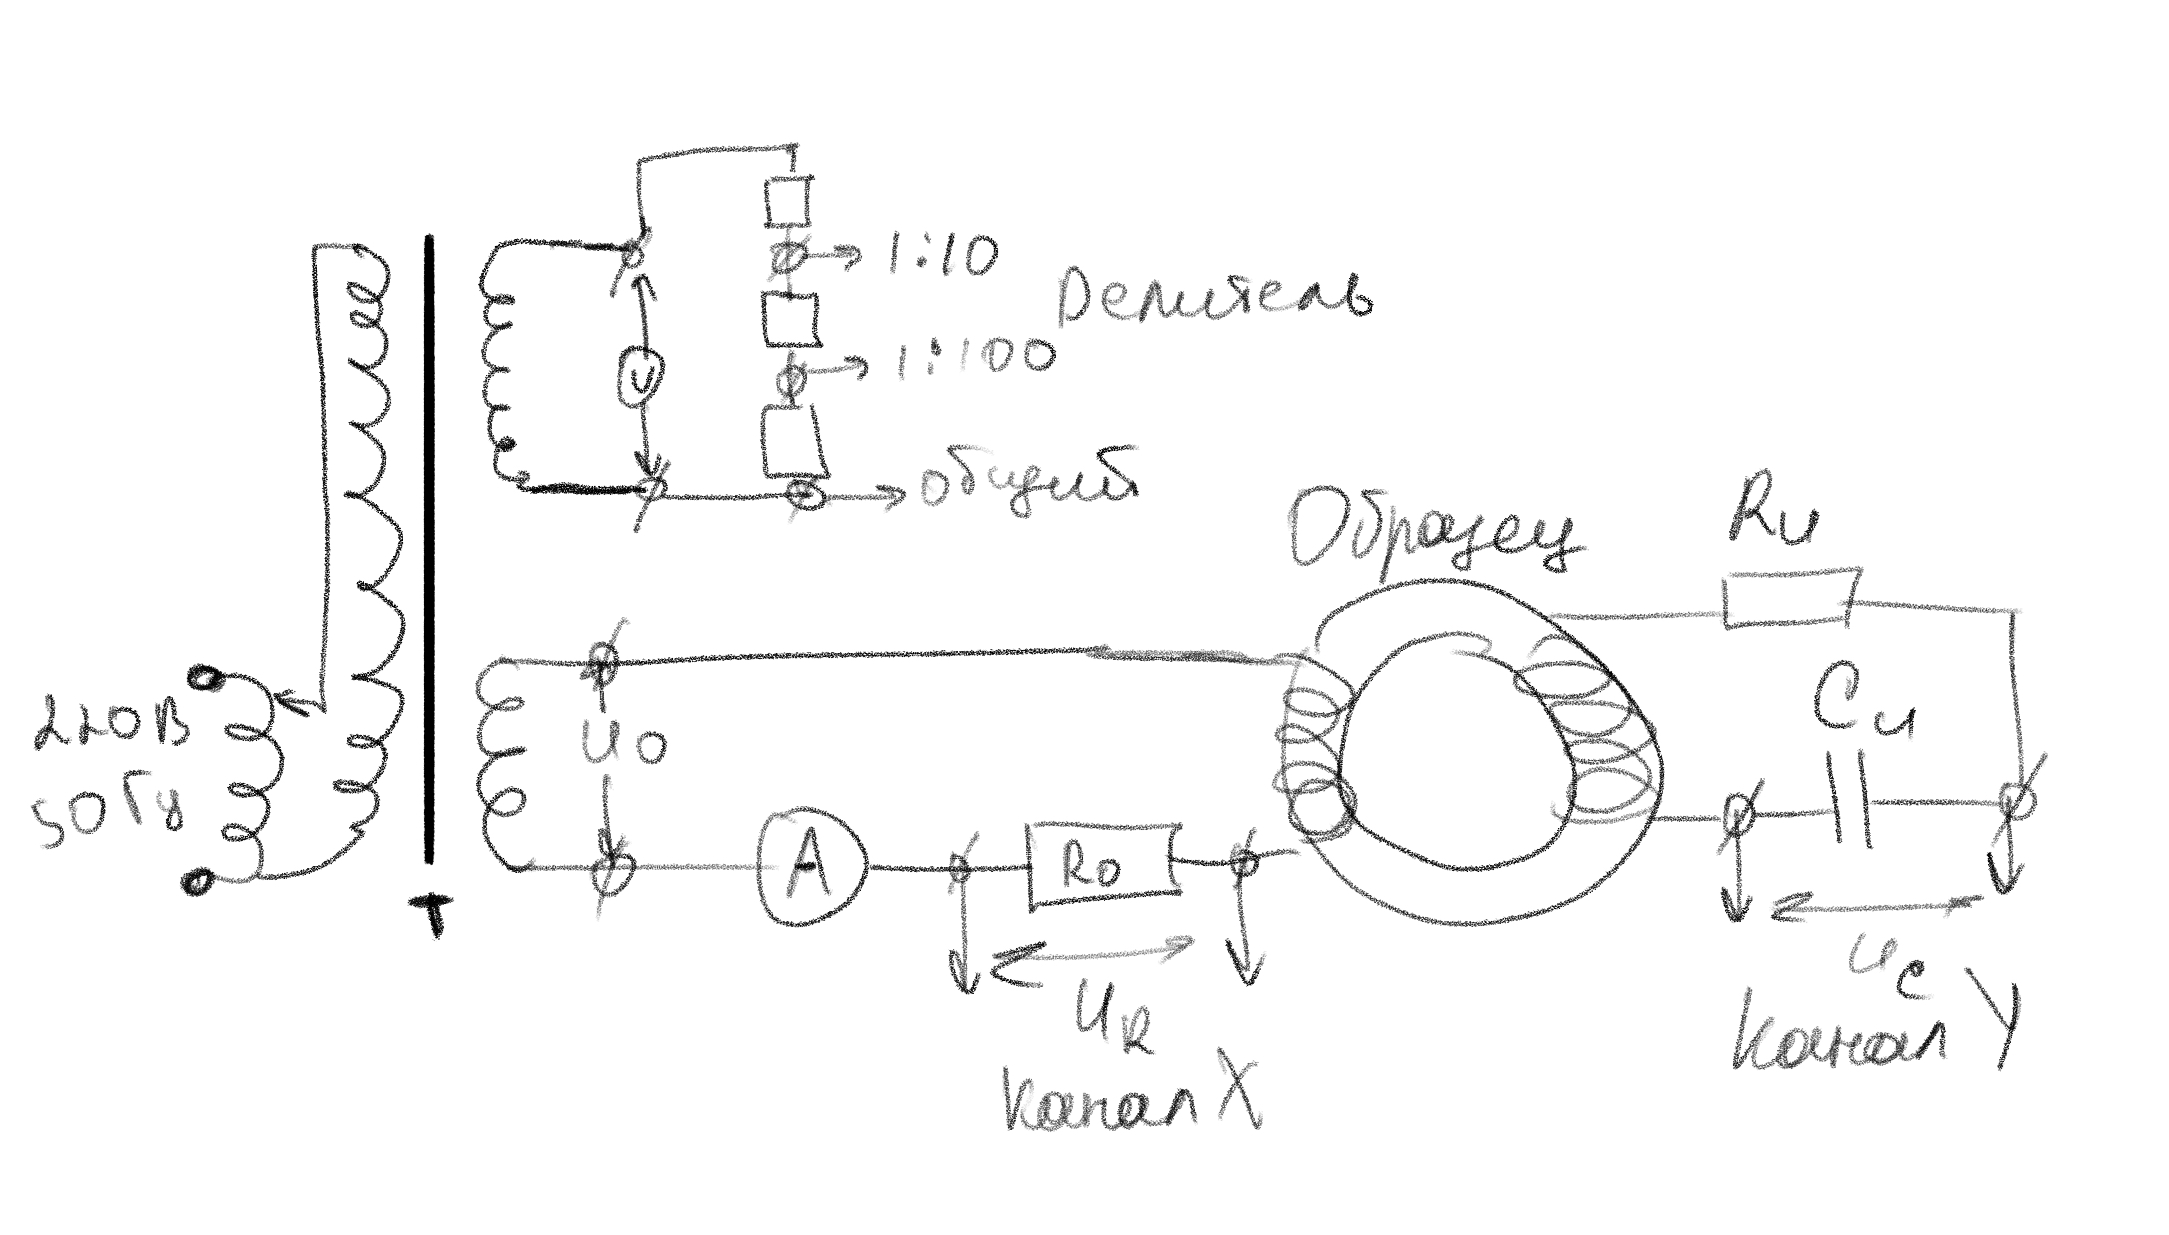
\includegraphics[width=1\textwidth]{set}
    \caption{Схема установки}
    \label{fig:set}
\end{figure}

\vspace{1 cm}

Схема установки представлена на рисунке \ref{fig:set}. Напряжение сети (220 В, 50 Гц) с помощью трансформаторного блока Т, состоящего из регулировочного автотрансформатора и 
разделительного понижающего трансформатора, подаётся на намагничивающую обмотку $N_0$ исследуемого образца.
В цепь намагничивающей катушки, на которую подаётся некоторое напряжение $V_0$, последовательно включено сопротивление $R_0$. Напряжение на $R_0$, 
равное $U_R = R_0I_0$, где $I_0$ - ток в намагничивающей обмотке $N_0$, подаётся на канал $X$ осциллографа. Связь напряжённости $H$ в
образце и тока $I_0$ рассчитывается по теореме о циркуляции. Действующее значение переменного тока в обмотке $N_0$ измеряется амперметром A.

Для измерения магнитной индукции $B$ с измерительной обмоткой $N_\text{вх}$, пропорциональное производной $dB/dt$. С интегрирующей
ёмкости $C_\text{и}$ снимается напряжение $U_\text{вых}$, пропорциональное величине $B$, и подается на вход $Y$ осциллографа. Значение индукции 
поля $B$ рассчитывается по формуле \ref{1}

\begin{equation}\label{1}
	|B| = \frac{1}{SN} \int\ U_\text{вх} dt = \frac{\tau_\text{и}}{SN}U_\text{вых},
\end{equation}
где $\tau_\text{и} = R_\text{и} C_\text{и}$ --- постоянная времени $RC$-цепочки.
Замкнутая кривая, возникающая на экране осциллографа, воспроизводит в масштабе петлю гистерезиса, который выбирается
вручную.

\section{Теоретические сведения}

К ферромагнетикам принадлежат железо, никель, кобальт, гадолиний,
их многочисленные сплавы с другими металлами. К ним примыкают ферриты --- диэлектрики
со структурой антиферромагнетика.

Магтнитная индукция \textbf{$B$} и напряженность магнитного поля 
\textbf{$H$} в ферромагнитном материале неоднозначно связаны между собой:
индукция зависит не только от напряженности, но и от предыстории образца.
Связь между индукцией и напряженностью поля типичного ферромагнетика 
иллюстрирует рисунок \ref{fig:gist}.

\begin{figure}[h]
    \centering
    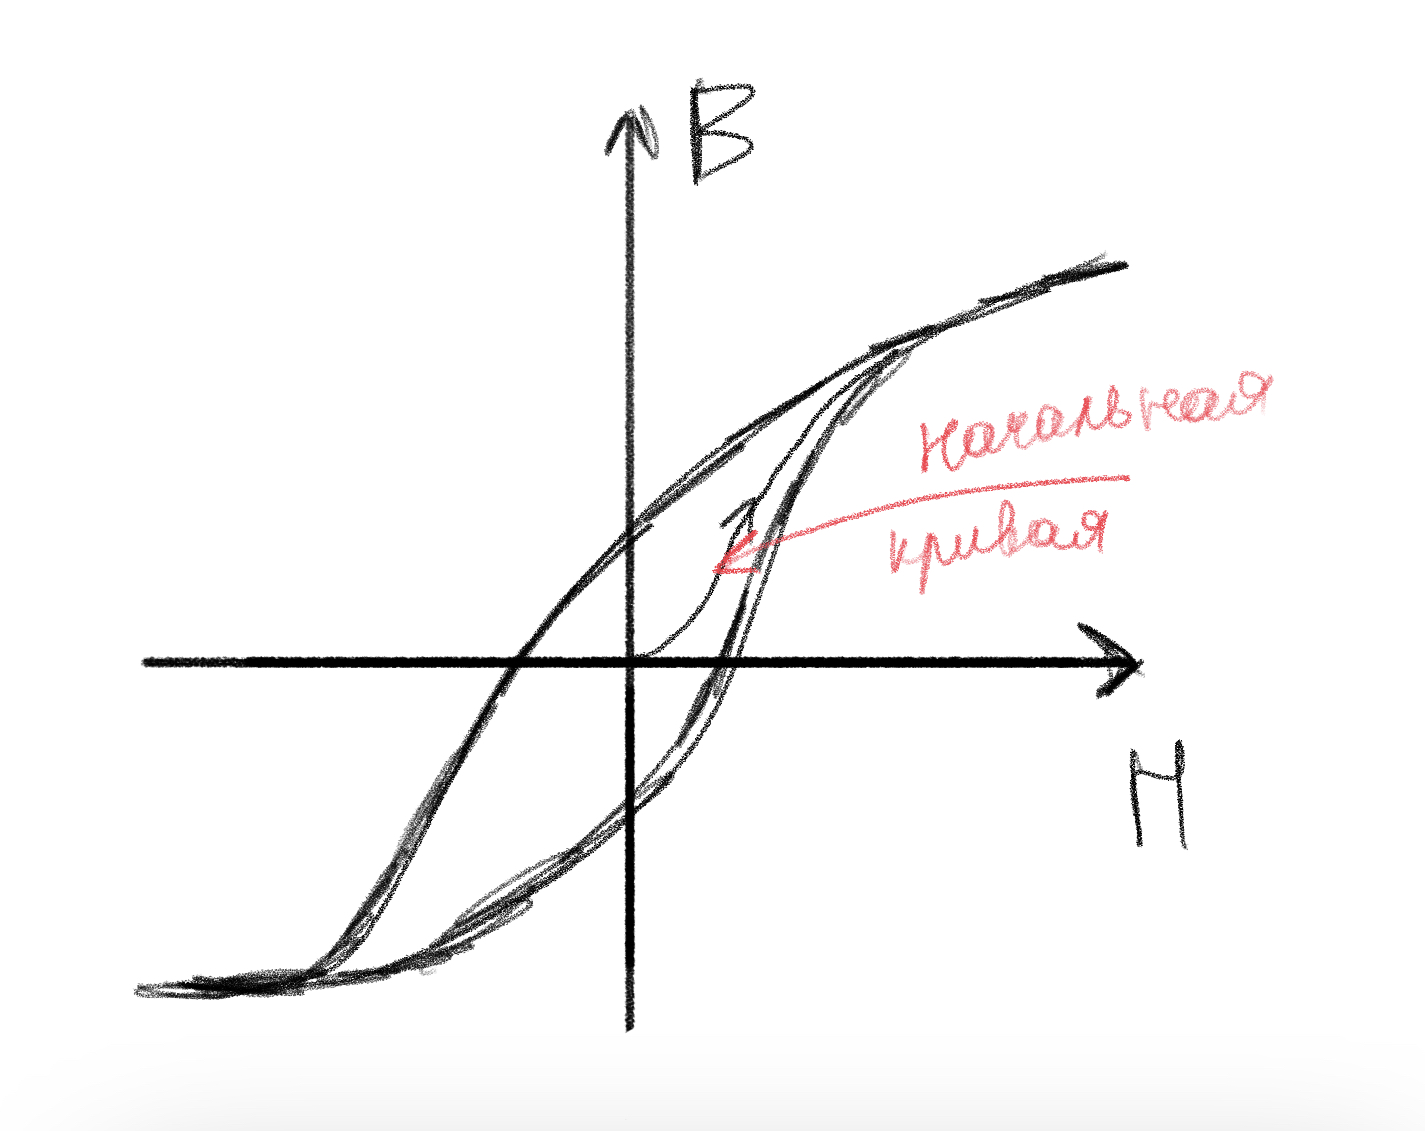
\includegraphics[width=0.8\textwidth]{gist}
    \caption{Петля гистерезиса}
    \label{fig:gist}
\end{figure}

\section{Обработка результатов}

Занесем характеристики образцов в таблицу \ref{tab:chartics}:

\begin{table}[H]
	\centering
	\begin{tabular}{|c|c|c|c|c|}
	\hline
	Материал & $N_0$ & $N_u$ & S, см & 2$\pi$R, см \\ \hline
	FeNi     & 35   & 220  & 3,8   & 24       \\ \hline
	FeSi     & 40   & 400  & 1,2   & 10       \\ \hline
	Ferrit   & 40   & 400  & 3     & 25       \\ \hline
	\end{tabular}
	\caption{Характеристики образцов}
	\label{tab:chartics}
	\end{table}

Для каждого из трех образцов будем подбирать коэффициенты усиления на осциллографе так, чтобы предельная
петля занимала большую часть экрана. Занесем в таблицу \ref{tab:axes} полные высоты предельной петли
$2X_s, 2Y_s$, соответствующие удвоенной амплитуде колебания напряженности $H_s$ и индукции $B_s$, а так же 
двойные амплитуды коэрцетивного поля и остаточной индукции:

\begin{table}[H]
	\centering
	\begin{tabular}{|c|c|c|c|c|}
	\hline
	Материал & {$2X_s$} & $2Y_s$ & $2X_c$ & $2Y_r$ \\ \hline
	FeNi                   & 5,2                      & 4,6 & 2,4 & 4,4 \\ \hline
	FeSi                   & 8,4                      & 5   & 1   & 2   \\ \hline
	Ferrit                 & 7,6                      & 2   & 0,8 & 2,4 \\ \hline
	\end{tabular}
	\caption{Характеристики предельной петли}
	\label{tab:axes}
\end{table}

Затем по формулам \ref{2} и \ref{3}

\begin{equation}\label{2}
	H = \frac{IR_0}{2 \pi R}
\end{equation}

\begin{equation}\label{3}
	B = \frac{R_\text{и} C_\text{и} U_\text{вых}}{S N_\text{и}}
\end{equation}

рассчитаем цену деления по каждой из осей для каждого образца. Результаты занесем в таблицу \ref{tab:tsena_deleniya}

\begin{table}[H]
	\centering
	\begin{tabular}{|c|c|c|}
	\hline
	Материал & H, А/м/дел & B, Тл/дел \\ \hline
	FeNi     & 24,3       & 0,48      \\ \hline
	FeSi     & 133,3      & 0,83      \\ \hline
	Ferrit   & 10,7       & 0,07      \\ \hline
	\end{tabular}
	\caption{Цены деления}
	\label{tab:tsena_deleniya}
	\end{table}

Теперь, зная цену деления можем найти двойные амплитудные значения предельной напряженности и индукции, 
а так же двойные амплитуды коэрцетивного поля и остаточной индукции:

\begin{table}[H]
	\centering
	\begin{tabular}{|c|c|c|c|c|}
	\hline
	Материал & 2H, А/м       & $\epsilon$ & 2B, Тл      & $\epsilon$ \\ \hline
	FeNi     & 126.36  & 0.10    & 2.20 & 0.11    \\ \hline
	FeSi     & 1119.72 & 0.06    & 4.15    & 0.10    \\ \hline
	Ferrit   & 81.32   & 0.07    & 0.14    & 0.24    \\ \hline
	\end{tabular}
	\caption{Амплитудные значения}
	\label{tab:amplitudi}
\end{table}

\begin{table}[H]
	\centering
	\begin{tabular}{|c|c|c|c|c|}
	\hline
	Материал & $2H_c$, А/м  & $\epsilon$ & $2B_s$, Тл   & $\epsilon$ \\ \hline
	FeNi     & 58.32  & 0.21       & 2.11 & 0.11       \\ \hline
	FeSi     & 133.30 & 0.50       & 1.66    & 0.25       \\ \hline
	Ferrit   & 8.56   & 0.62       & 168.00  & 0.20       \\ \hline
	\end{tabular}
	\caption{Амплитудные значения коэрц. поля и ост. индукции}
	\label{tab:koerc}
\end{table}

Для сравнения приведем табличные данные:

\begin{table}[H]
	\centering
	\begin{tabular}{|c|c|c|}
		\hline
		Материал     & $H_c$, А/м & $B_s$, Тл \\ \hline
		FeNi         & 11--40     & 1,51      \\ \hline
		Fesi         & 50--100    & 1,21      \\ \hline
		Ferrit       & 20         & 0,27      \\ \hline
	\end{tabular}
	\caption{Табличные данные}
	\label{tab:tablica}
\end{table}

\section{Приложение}

Графики начальных кривых намагничивания:

\begin{figure}[h]
    \centering
    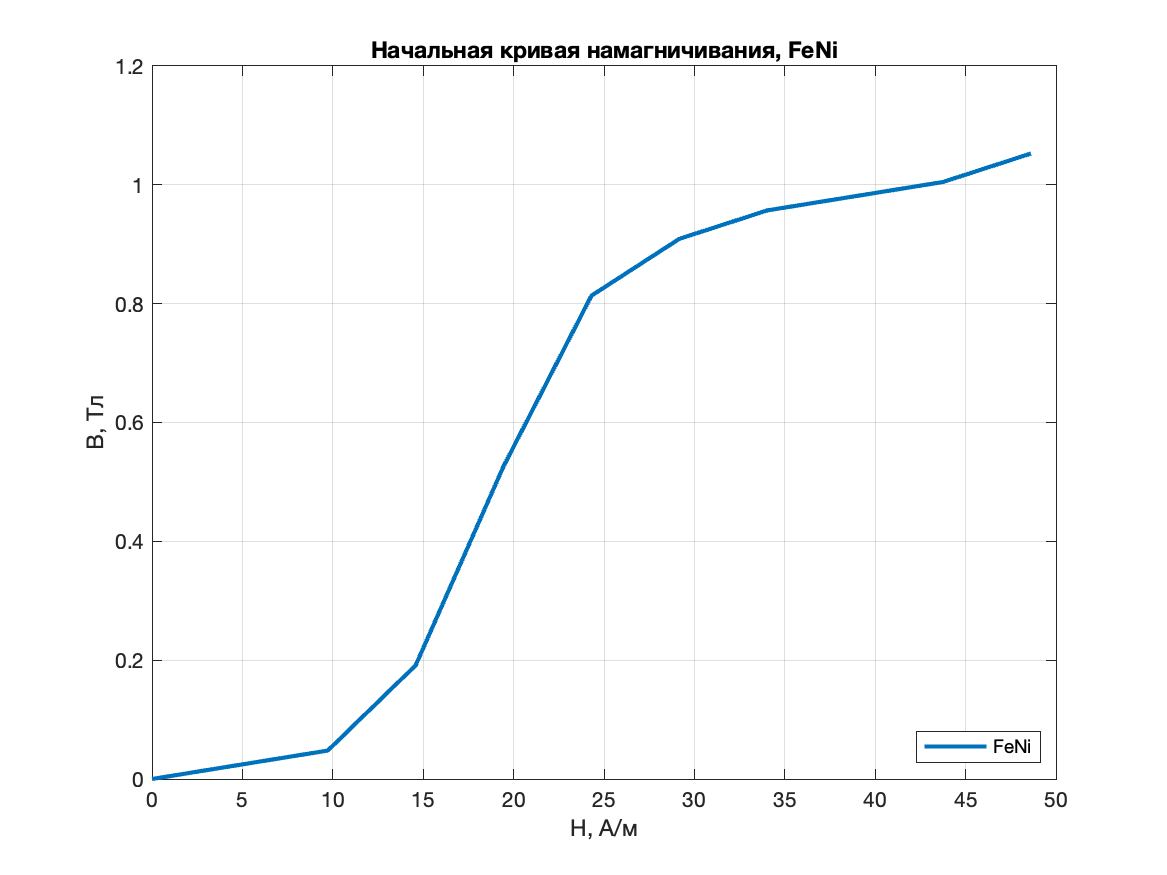
\includegraphics[width=0.8\textwidth]{FeNi}
    \caption{Начальная кривая FeNi}
    \label{fig:FeNi}
\end{figure}

\begin{figure}[h]
    \centering
    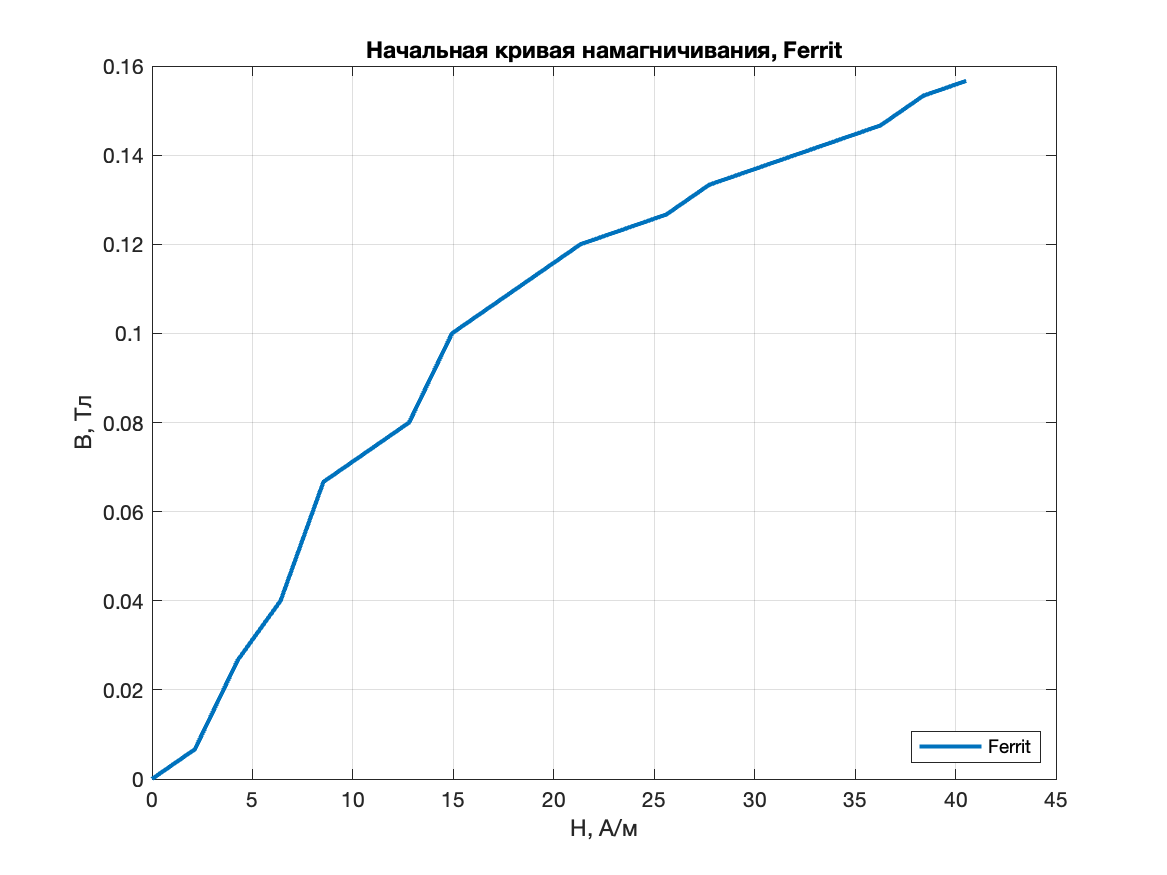
\includegraphics[width=0.8\textwidth]{Ferrit}
    \caption{Начальная кривая Ferrit}
    \label{fig:Ferrit}
\end{figure}

\begin{figure}[h]
    \centering
    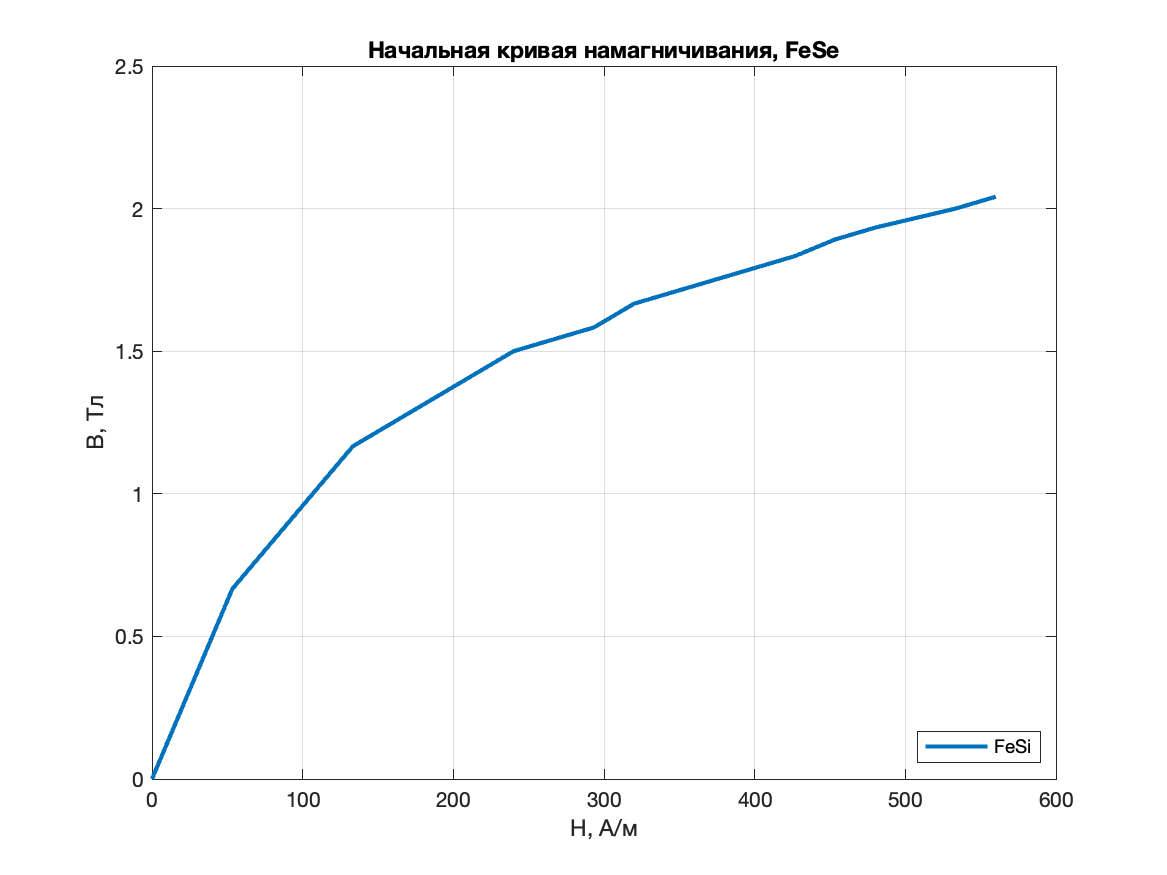
\includegraphics[width=0.8\textwidth]{FeSi}
    \caption{Начальная кривая FeSi}
    \label{fig:FeSi}
\end{figure}

\end{document}